\documentclass[12pt]{article}

\setlength\parindent{0pt}
\newcommand{\myt}[1]{\textbf{\underline{#1}}}

\usepackage{mathtools}
\usepackage{amssymb}

\usepackage{tikz,ifthen,amsmath,amssymb,fancyhdr,comment,lastpage}

\title{\vspace{-15ex}Tutorial 6 CS 241\vspace{-1ex}}
\date{June 19th, 2015}
\author{Graham Cooper}

\begin{document}
	\maketitle
	
	Topics\\
	- Non-deterministic Finite Automata (NFAs)\\
	- Context Free Languages (CFLs)\\
	
	\section*{NFAS}
	\begin{itemize}
		\item $\Sigma$ - input alphabet
		\item Q - finite set of states
		\item $q_0 \in Q$ - starting state
		\item A $\subseteq$ Q - set of accepting states
		\item $\delta$: Q $\times \Sigma \rightarrow 2^Q$ - transition function
		\item $\delta$: Q $\times \Sigma \rightarrow$ Q
	\end{itemize}
	
	\section*{CFGs}
	\begin{itemize}
		\item $\Sigma/T$ - finite set of terminals
		\item V/N - finite set of non-terminals
		\item P/R - finite set of rewrite/production rules
		\item S - starting non-terminal
	\end{itemize}
	
	\section*{NFA Problems}
	
	\subsection*{1)}
	$\Sigma \{a,b,c\}$\\
	L = \{Strings ending in abc or cab\}\\
	
	See page for image
	
	\subsection*{2)}
	Convert the previous NFA to a DFA using subset construction\\
	
	See page for image
	
	\section*{CFL Problems}
	
	\subsection*{1)}
	Write a CFG that generates the same language as the NFA\\
	
	S $\rightarrow$ abc $|$ cab $|$ TS\\
	T $\rightarrow$ a$|$b$|$c\\
	
	\subsection*{2)}
	$\Sigma \{0,1\}$\\
	L = $\{0^n1^n | n \geq 0 \}$\\
	
	S $\rightarrow$ $\epsilon | $ 0S1\\
	
	\subsection*{4)}
	$S \rightarrow f(A)$\\
	$S \rightarrow g(A,A)$\\
	$A \rightarrow x$\\
	$A \rightarrow y$\\
	$A \rightarrow S$\\
	f(x)\\
	g(y,f(x))\\
	f(g(g(x,y,f(x))))\\
	
	g(f(x), g(x,y))\\
	
	$$S \implies_2 g(A,A)$$
	$$\implies_5 g(S,A)$$
	$$\implies_1 g(f(A), A)$$
	$$\implies_3 g(f(x), A)$$
	$$\implies_5 g(f(x), S)$$
	$$\implies_2 g(f(x), g(A,A)$$
	$$\implies_3 g(f(x), g(x, A)$$
	$$\implies_4 g(f(x), g(x,y))$$
	
	\begin{center}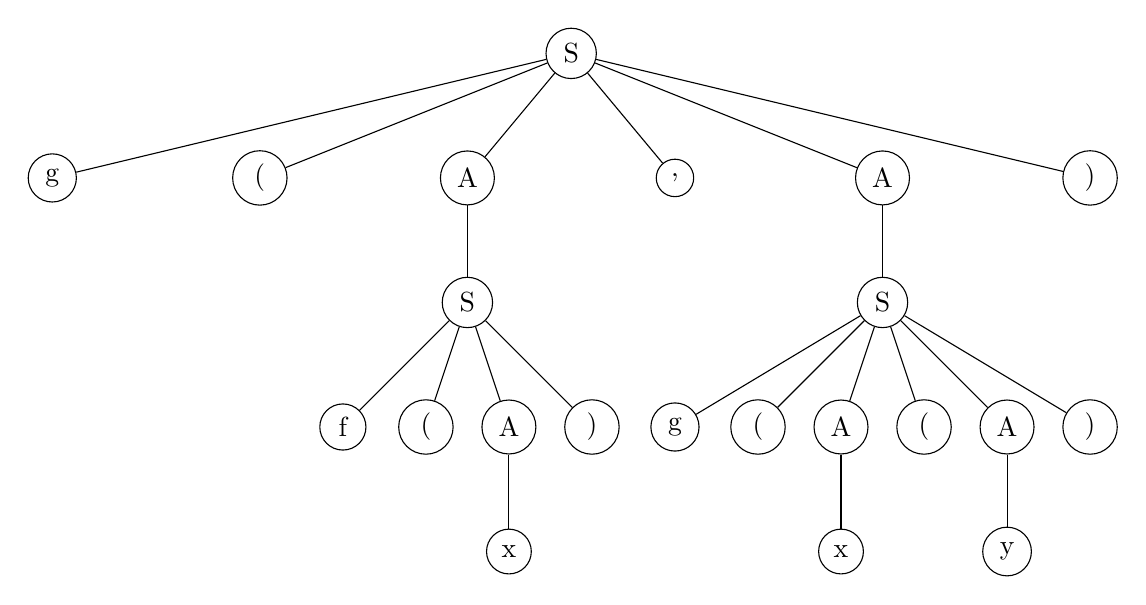
\begin{tikzpicture}[
		level distance=45 pt,
		every node/.style={circle,draw},
		level 1/.style={sibling distance=75 pt},
		level 2/.style={sibling distance=50 pt},
		level 3/.style={sibling distance=30 pt}
		]
		\node {S}
		child {node {g}}
		child {node {(}}
		child {node {A}
			child {node {S}
				child {node {f}}
				child {node {(}}
				child {node {A}
					child {node {x}}
				}
				child {node {)}}
			}
		}
		child {node {,}}
		child {node {A}
			child {node {S}
				child {node {g}}
				child {node {(}}
				child {node {A}
					child {node {x}}
				}
				child {node {(}}
				child {node {A}
					child {node {y}}
				}
				child {node {)}}
			}
		}
		child {node {)}}
		;
	\end{tikzpicture}\end{center}

	\subsection*{5)}
	
	\begin{itemize}
		\item S $\rightarrow$ (S)
		\item S $\rightarrow$ SS
		\item S $\rightarrow \epsilon$	
	\end{itemize}
	
	Very helpful for assignment question!!!\\
	
	\begin{verbatim}
	eval(tree)
	-- if (rule == s -> e) return 0
	-- else if (rule == s -> (S)) return 1 + eval(S)
	-- else if (rule == S -> S1S2) return max (eval(S1), eval(S2))
	\end{verbatim}
	
	
	
	
\end{document}
